
\section{Test Problems}
\label{sec:problems}

% {\bf For each test problem: a) clearly state the mathematical problem,
% linking the notation to that in subsection \ref{ssec:PS};
% b) clearly state specifics of the architecture that you will make
% for this specific test problem, linking the notation to that in subsection \ref{ssec:PA}.}

A central application of neural operators is learning solution operators defined by parametric partial differential equations. In this section, we define four test problems for which we numerically study the approximation properties of neural operators. To that end, let \((\A,\U,\mathcal{F})\) be a triplet of Banach spaces. The first two problem classes considered are derived from the following general class of PDEs: 
\begin{align}
\label{eq:generalpde}
\begin{split}
\LL_a u &= f
\end{split}
\end{align}
where, for every \(a \in \A\), \(\LL_a : \U \to \mathcal{F}\) is a, possibly nonlinear, partial differential operator, and \(u \in \U\) corresponds to the solution of the PDE \eqref{eq:generalpde} when \(f \in \mathcal{F}\) and appropriate boundary conditions are imposed.
The second class will be evolution equations with initial
condition \(a \in \A\) and solution \(u(t) \in \U\) at every time $t>0.$
We seek to learn the map from $a$ to $u:=u(\tau)$
for some fixed time $\tau>0;$ we will also study maps on 
paths (time-dependent solutions).

Our goal will be to learn the mappings
\[\Ftrue: a \mapsto u \qquad \text{or} \qquad \Ftrue : f \mapsto u;\]
we will study both cases, depending on the test problem considered. We will define a probability measure \(\mu\) on \(\A\) or \(\mathcal{F}\) which will serve to define a model for likely input data. Furthermore, measure \(\mu\) will define a topology on the space of mappings in which \(\Ftrue\) lives, using the Bochner norm \eqref{eq:bochner_error}. 
We will assume that each of the spaces \((\A,\U,\mathcal{F})\) are Banach spaces of functions defined on a bounded domain \(D \subset \R^d\). All reported errors will be Monte-Carlo estimates of the relative error
\[\mathbb{E}_{a \sim \mu} \frac{\|\Ftrue(a) - \G_\theta(a)\|_{L^2(D)}}{\|\Ftrue (a)\|_{L^2(D)}}\]
or equivalently replacing \(a\) with \(f\) in the above display and with the assumption that \(\U \subseteq L^2(D)\). The domain $D$ will be discretized,  usually uniformly, with $J \in \N$ points. 

\subsection{Poisson Equation}
\label{ssec:poisson}
First we consider the one-dimensional Poisson equation with a zero boundary condition.
In particular, \eqref{eq:generalpde} takes the form
\done{I prefer to make operator positive; please make any changes
needed from the sign-change}
\begin{align}
\label{eq:poisson}
\begin{split}
    -\frac{d^2}{dx^2} u(x) &= f(x),  \qquad x \in (0,1)\\
    u(0) = u(1) &= 0
\end{split}
\end{align}
for some source function \(f: (0,1) \to \R)\). In particular, for \(D(\LL):=H^1_0((0,1);\R) \cap H^2((0,1);\R)\), we have \(\LL: D(\LL) \to L^2((0,1);\R)\) defined as $-d^2/dx^2$, noting that 
that $\LL$ has no dependence on any parameter \(a \in \A\) in this case. We will consider the weak form of \eqref{eq:poisson} with source function \(f \in H^{-1}((0,1);\R)\) and therefore the solution operator  \(\Ftrue : H^{-1}((0,1);\R) \to H^1_0((0,1);\R)\) defined as
\[\Ftrue: f \mapsto u.\]
We define the probability measure \(\mu = N(0,C)\) where
\[C = \Bigl ( \LL + I \Bigl)^{-2},\]
defined through the spectral theory of self-adjoint operators.  Since \(\mu\) charges a subset of \(L^2((0,1);\R)\), we will learn \(\Ftrue : L^2((0,1);\R) \to H^1_0((0,1);\R)\) in the topology induced by \eqref{eq:bochner_error}.

In this setting, \(\Ftrue\) has a closed-form solution given as
\[\Ftrue(f) = \int_0^1 G(\cdot,y) f(y) \: \text{d}y\]
where
\[G(x,y) = \frac{1}{2} \left ( x + y - |y-x| \right ) - xy, \qquad \forall (x,y) \in [0,1]^2\]
is the Green's function. Note that while \(\Ftrue\) is a linear operator, the Green's function \(G\) is non-linear
as a function of its arguments. We will consider only a single layer of \eqref{eq:F} with \(\sigma_1 = \text{Id}\), \(\cP = \text{Id}\), \(\cQ = \text{Id}\), \(W_0 = 0\), \(b_0 = 0\), and 
\[\mathcal{K}_0(f) = \int_0^1 \kappa_{\theta} (\cdot,y) f(y) \: \text{d}y\]
where \(\kappa_\theta : \R^2 \to \R\) will be parameterized as a standard neural network with parameters \(\theta\).

The purpose of the current example is two-fold. First we will test the efficacy of the neural operator framework in a simple setting where an exact solution is analytically available. Second we will show that by building in the right inductive bias, in particular, paralleling the form of the Green's function solution, we obtain a model that generalizes outside the distribution \(\mu\). That is, once trained, the model will generalize to any \(f \in L^2((0,1);\R)\) that may be outside the support of \(\mu\). For example, as defined, the random variable \(f \sim \mu\) is a continuous function, however, if \(\kappa_\theta\) approximates the Green's function well then the model \(\Ftrue\) will approximate the solution to \eqref{eq:poisson} accurately even for discontinuous inputs. 



To create the dataset used for training, solutions to \eqref{eq:poisson} are obtained by numerical integration using the Green's function on a uniform grid with \(85\) collocation points. We use \(N = 1000\) training examples. 

\iffalse
The 1d poisson equation has a well-defined Green function formation. We want to visualize the learn kernel function $\kappa$ and compared it with the true underlying Green function kernel. Now consider the setting where \(D = [0,1]\), $\LL_a = \partial_{xx}$, so that \eqref{eq:generalpde} reduces to the 1-dimensional Poisson equation.

where $f: [0,1] \to \R$ is the source function; $u: [0,1] \to \R$ is the solution function. The goal is to learn the map 
\[\Ftrue: f \mapsto u\]
The data is generated on a $85 \times 85$ grid. We set the number of training data to be $1000$; the number of testing data to be $1000$ as well.


\paragraph{Green's function.}
The above equation has an explicit Green's function:
\[G(x,y) = \frac{1}{2} \left ( x + y - |y-x| \right ) - xy. \]
such that 
\[u(x)  = \int_0^1 G(x,y) f(y) \mathrm{d}y\]

Note that although the map \(\Ftrue: f \mapsto u\) is, in function space, linear,  the Green's function itself is not linear in either argument.

For this problem,
we consider a simplification of the iterative update framework defined in section \ref{sec:framework}. We omit step 1.,2. and 4. and only use one iteration of step 3. In other words, we set \(v_0(x) = f(x)\), \(T=1\), \(n=1\), \(\sigma(x) = x\), \(W = w = 0\), and \(\nu_x(dy) = dy\) (the Lebesgue measure). The purposed operator $\cF$ can be directly written as
\[(\cF f)(x) = \int_0^1 \kappa(x,y; \phi) f(y) \mathrm{d}y \]
For this test problem, we want to show whether the neural network $\kappa$ will match the Green function $G$.
\fi

\subsection{Darcy Flow}
\label{ssec:darcy}
We consider the steady state of Darcy Flow in two dimensions which is the second order elliptic equation
\begin{align}
\label{eq:darcy}
\begin{split}
- \nabla \cdot (a(x) \nabla u(x)) &= f(x), \qquad x \in D \\
u(x) &= 0, \qquad \quad \:\: x \in \partial D
\end{split}
\end{align}
where \(D = (0,1)^2\) is the unit square. In this setting \(\A = L^\infty(D;\R_+)\), \(\U = H_0^1(D;\R)\), and \(\mathcal{F} = H^{-1}(D;\R)\).
We fix \(f \equiv 1\) and consider the weak form of \eqref{eq:darcy} and therefore the solution operator \(\Ftrue : L^\infty(D;\R^+) \to H^1_0(D;\R)\) defined as
\begin{equation}
    \label{eq:darcysolutionop}
    \Ftrue:  a \mapsto u.
\end{equation}
Note that while \eqref{eq:darcy} is a linear PDE, the solution operator \(\Ftrue\) is nonlinear. We define the probability measure \(\mu = T_\sharp N(0,C)\) \nk{as the pushforward of a Gaussian measure under the operator \(T\)} where \nk{the covariance of the Gaussian is}
\[C = (-\Delta + 9I)^{-2}\]
with $D(-\Delta)$ defined to impose zero Neumann boundary on the Laplacian. We 
\nk{define} \(T\) to be a Nemytskii operator acting on functions, defined through the map \(T : \R \to \R_+\) defined as
\[T(x) = \begin{cases}
12, & x \geq 0 \\
3, & x < 0
\end{cases}.\]
The random variable \(a \sim \mu\) is a piecewise-constant function with random interfaces given by the underlying Gaussian random field. Such constructions are prototypical models for many physical systems such as permeability in sub-surface flows and (in a vector
generalization) material microstructures in elasticity. 

To create the dataset used for training, solutions to \eqref{eq:darcy} are obtained using a second-order finite difference scheme on a uniform grid of size \(421 \times 421\). All other resolutions are downsampled from this data set. We use \(N = 1000\) training examples.

\iffalse
The coefficients $a$ are generated according to \(a \sim \mu \) where \(\mu = \psi_{\#} \mathcal{N}(0,(-\Delta + 9I)^{-2})\)
with a Neumann boundry condition on the operator \(-\Delta + 9I\) and $f(x)$ is fixed.
The mapping \(\psi : \R \to \R\) takes the value $12$ on the positive part of the real line and $3$ on the negative. Such constructions are prototypical models for many physical systems such as permeability in sub-surface flows and material microstructures in elasticity. Solutions \(u\) are obtained by using a second-order finite difference scheme on $241 \times 241$ and $421 \times 421$ grids. Different resolutions are downsampled from this dataset. 
Without specific notice, the number of training data is set to be $1000$; the number of testing data to be $100$.
For this problem we want to learn the operator for the coefficient function $a$ to the solution function $u$:
\[\Ftrue: a \mapsto u\]
\fi


\subsection{Burgers' Equation}
\label{ssec:burgers}
We consider the one-dimensional viscous Burgers' equation
\begin{align}
    \label{eq:burgers}
    \begin{split}
    \frac{\partial}{\partial t} u(x,t) + \frac{1}{2} \frac{\partial}{\partial x} \bigl ( u(x,t) \bigl)^2 &= \nu \frac{\partial^2}{\partial x^2} u(x,t), \qquad x \in (0,2\pi), t \in (0,\infty) \\
    u(x,0) &= u_0(x), \qquad \qquad \:\:\: x \in (0,2\pi)
    \end{split}
\end{align}
with periodic boundary conditions and a fixed viscosity \(\nu = 10^{-1}\). Let \(\Psi : L^2_{\text{per}}((0,2\pi);\R) \times \R_+ \to H^s_{\text{per}}((0,2\pi);\R)\), for any \(s > 0\), be the flow map associated to \eqref{eq:burgers}, in particular,
\[\Psi(u_0, t) = u(\cdot,t), \qquad t > 0.\]
We consider the solution operator defined by evaluating \(\Psi\) at a fixed time. Fix any $s \ge 0.$ Then we may define \(\Ftrue : L^2_{\text{per}}((0,2\pi);\R) \to H^s_{\text{per}}((0,2\pi);\R)\) by
\begin{equation}
    \label{eq:burgerssolutionop}
    \Ftrue : u_0 \mapsto \Psi(u_0,1).
\end{equation}
We define the probability measure \(\mu = N(0,C)\) where
\[C = 625 \Bigl ( -\frac{d^2}{dx^2} + 25I \Bigl)^{-2}\]
with domain of the Laplacian defined to impose periodic boundary conditions. We chose the initial condition for \eqref{eq:burgers} by drawing \(u_0 \sim \mu\), noting that \(\mu\) charges a subset of \(L^2_{\text{per}}((0,2\pi);\R)\).

To create the dataset used for training, solutions to \eqref{eq:burgers} are obtained using a pseudo-spectral split step method where the heat equation part is solved exactly in Fourier space and then the non-linear part is advanced using a forward Euler method with a very small time step. We use a uniform spatial grid with \(2^{13} = 8192\) collocation points and subsample all other resolutions from this data set. We use \(N = 1000\) training examples.


\iffalse
We consider mapping the initial condition to the solution at time one \(u_0 \mapsto u(\cdot, 1)\). The initial condition is generated according to 
\(u_0 \sim \mu\) where \(\mu = \mathcal{N}(0,625(-\Delta + 25I)^{-2})\) with periodic boundary conditions. We set the viscosity to \(\nu = 0.1\) and solve the equation using a split step method where the heat equation part is solved exactly in Fourier space and then the non-linear part is advanced, again in Fourier space, using a very fine forward Euler method. We solve on a spatial mesh with resolution $2^{13} = 8192$ and use this dataset to subsample other resolutions. Unless we specify otherwise, the number of training data is set to be $1000$; the number of testing data to be $100$.
Again, we want to learn the operator for the coefficient function $a$ to the solution function $u$:
\[\Ftrue: u|_{t=0} \mapsto u|_{t=1}\]
\fi 

\subsection{Navier-Stokes Equation}
\label{ssec:nse}

\done{I am worried about this formulation of the equation. I'd rather
you formulate the equation in velocity space, define the vorticity,
and simply mention that there is an equation for the vorticity
which can be solved directly. Look at how Chandler-Kerswell write it.
(But use $\Delta$ not $\nabla^2$!
The point of using streamfunction is that it automatically
imposes divergence free; and then vorticity is related to it
by Laplacian so same thing applies. Is the forcing as stated
the forcing in vorticity space? More natural to define forcing
in velocity space.}

We consider the two-dimensional Navier-Stokes equation for a viscous, incompressible fluid 
\begin{align}
\label{eq:navierstokes-velocity}
\begin{split}
\partial_t u(x,t) + u(x,t) \cdot \nabla u(x,t) + \nabla p(x,t) &= \nu \Delta u(x,t) + f(x), \qquad x \in \mathbb{T}^2, t \in (0,\infty)  \\
\nabla \cdot u(x,t) &= 0, \qquad \qquad \qquad \qquad \:\:\: x \in \mathbb{T}^2, t \in [0,\infty)  \\
u(x,0) &= u_0(x), \qquad \qquad \qquad \:\:\: x \in \mathbb{T}^2 
\end{split}
\end{align}
where \(\mathbb{T}^2\) is the unit torus i.e. \([0,1]^2\) equipped with periodic boundary conditions, and \(\nu \in \R_+\) is a fixed viscosity.
Here $u : \mathbb{T}^2 \times \R_+ \to \R^2$ is the velocity field,  
$p : \mathbb{T}^2 \times \R_+ \to \R^2$ is the pressure field, and
 \(f: \mathbb{T}^2 \to \R\) is a fixed forcing function.


Equivalently, we study the vorticity-streamfunction formulation of the equation
% {\bf equations under construction}\\
\begin{subequations}
\label{eq:navierstokes}
\begin{align}
\partial_t w(x,t) + \nabla^{\perp}\psi \cdot \nabla w(x,t) &= \nu \Delta w(x,t) + g(x), \qquad x \in \mathbb{T}^2, t \in (0,\infty),  \\
-\Delta \psi&=\omega, \qquad\qquad\qquad\qquad\:\:\: x \in \mathbb{T}^2, t \in (0,\infty),  \\
 w(x,0) &= w_0(x), \qquad \qquad \qquad \:\:\: x \in \mathbb{T}^2, 
\end{align}
\end{subequations}
where \(w\) is the out-of-plane component of the vorticity field \(\nabla \times u: \mathbb{T}^2 \times \R_+ \to \R^3\). Since, when viewed in three dimensions, 
$u=\bigl(u_1(x_1,x_2),u_2(x_1,x_2),0\bigr)$, it follows that
$\nabla \times u=(0,0,\omega).$ 
The stream function $\psi$ is related to the velocity by 
$u=\nabla^{\perp}\psi$, enforcing the divergence-free condition.
Similar considerations as for the curl of $u$ apply to the curl of $f$, 
showing that $\nabla \times f=(0,0,g).$
\nk{Note that in (\ref{eq:navierstokes}b) $\psi$ is undetermined up to an (irrelevant, since $u$ is computed from $\psi$ by taking a gradient) additive constant; uniqueness is restored
by seeking $\psi$ with spatial mean $0.$}
 We define the forcing term as
\[g(x_1,x_2) = 0.1(\sin(2\pi(x_1+x_2)) + \cos(2\pi(x_1 + x_2))), \qquad \forall (x_1,x_2) \in \mathbb{T}^2.\]
 The corresponding Reynolds number is estimated as 
 $Re = \frac{\sqrt{0.1}}{\nu (2 \pi)^{3/2}}$ \citep{chandler2013invariant}.
Let \(\Psi : L^2(\mathbb{T}^2;\R) \times \R_+ \to H^s(\mathbb{T}^2;\R)\), for any \(s > 0\), be the flow map associated to \eqref{eq:navierstokes}, in particular,
\[\Psi(w_0,t) = w(\cdot,t), \qquad t > 0.\]
Notice that this is well-defined for any \(w_0 \in L^2(\mathbb{T};\R)\). 
%We can see this through the stream-function formulation where the stream-function satisfies
%\[-\Delta \varphi_0(x) = w_0(x), \qquad \forall x \in \mathbb{T}^2\]
%and the initial velocity is defined as
%\[u(x,0) = \nabla^\perp \varphi_0(x), \qquad \forall x \in \mathbb{T}^2\]
%hence
%\[\nabla \cdot u(\cdot,0) =  \nabla \cdot \nabla^\perp \varphi_0 = 0\]
%is divergence free.

We will define two notions of the solution operator. In the first, we will proceed as in the previous examples, in particular, \(\Ftrue : L^2(\mathbb{T}^2;\R) \to H^s(\mathbb{T}^2;\R)\) is defined as
\begin{equation}
\label{eq:nssolutionop_add}
\Ftrue : w_0 \mapsto \Psi(w_0, T)
\end{equation}
for some fixed \(T > 0\). In the second, we will map an initial part of the trajectory to a later part of the trajectory. In particular, we define
\(\Ftrue : L^2(\mathbb{T}^2;\R) \times C \bigl ( (0,10]; H^s(\mathbb{T}^2;\R) \bigl) \to C \bigl( (10,T]; H^s(\mathbb{T}^2;\R) \bigl)\) by
\begin{equation}
    \label{eq:nssolutionop2}
    \Ftrue : \bigl ( w_0, \Psi(w_0,t)|_{t \in (0,10]} \bigl) \mapsto \Psi(w_0,t)|_{t \in (10,T]}
\end{equation}
for some fixed  \(T > 10\). We define the probability measure \(\mu = N(0,C)\)
where 
\[C = 7^{3/2}  (-\Delta + 49I)^{-2.5} \]
with periodic boundary conditions on the Laplacian. We model the initial vorticity \(w_0 \sim \mu\) to \eqref{eq:navierstokes} as \(\mu\) charges a subset of \(L^2(\mathbb{T}^2;\R)\).
Its pushforward onto $\Psi(w_0,t)|_{t \in (0,10]}$ is required to define the measure on
input space in the second case defined by \eqref{eq:nssolutionop2}.

To create the dataset used for training, solutions to \eqref{eq:navierstokes} are obtained using a pseudo-spectral split step method where the viscous terms are advanced using a Crank–Nicolson update and the nonlinear and forcing terms are advanced using Heun's method. Dealiasing is used with the \(2/3\) rule. For further details on this approach see \citep{chandler2013invariant}. Data is obtained on a uniform \(256 \times 256\) grid and all other resolutions are subsampled from this data set. We experiment with different viscosities \(\nu\), final times \(T\), and amounts of training data \(N\).

\iffalse
for any $r>0$ is the velocity field, $w = \nabla \times u$ is the vorticity, $w_0 \in L^2_{\text{per}}((0,1)^2;\R)$ is the initial vorticity,  $\nu \in \R_+$ is the viscosity coefficient, and $f \in L^2_{\text{per}}((0,1)^2;\R)$ is the forcing function. We are interested in learning the operator mapping the vorticity up to time 10 to the vorticity up to some later time $T > 10$,
$\Ftrue: C([0,10]; H^r_{\text{per}}((0,1)^2; \R)) \to C((10,T]; H^r_{\text{per}}((0,1)^2; \R))$
defined by 
\[\Ftrue: w|_{t \in [0,10]} \mapsto w|_{t \in (10,T]}\]

We choose to formulate the problem in terms of vorticity. Given the vorticity it is easy to derive the velocity. By formulating the problem on vorticity, the neural network models mimic the pseudo-spectral method. 
The initial condition $ w_0(x)$ is generated according to 
\(w_0 \sim \mu\) where \(\mu = \mathcal{N}(0,7^{3/2}(-\Delta + 49I)^{-2.5})\) with periodic boundary conditions. The forcing is kept fixed $f(x) = 0.1(\sin(2\pi(x_1+x_2)) + \cos(2\pi(x_1 + x_2)))$. The equation is solved using the stream-function formulation with a pseudospectral method. First a Poisson equation is solved in Fourier space to find the velocity field. Then the vorticity is differentiated and the non-linear term is computed is physical space after which it is dealiased. Time is advanced with a Crank–Nicolson update where the non-linear term does not enter the implicit part. 
All data are generated on a $256 \times 256$ grid and are downsampled to $64 \times 64$. We use a time-step of $1\mathrm{e}{-4}$ for the Crank–Nicolson scheme in the data-generated process where we record the solution every $t=1$ time units. 
We experiment with the viscosities $\nu = 1\mathrm{e}{-3}, 1\mathrm{e}{-4}, 1\mathrm{e}{-5}$, decreasing the final time $T$ as the dynamic becomes chaotic.
\fi

\subsubsection{Bayesian Inverse Problem}
\label{sec:problem:bayesian}

As an application of operator learning, we consider the inverse problem of recovering the initial vorticity in the Navier-Stokes equation \eqref{eq:navierstokes} from partial, noisy observations of the vorticity at a later time. Consider the first solution operator defined in subsection~\ref{ssec:nse}, in particular, \(\Ftrue : L^2(\mathbb{T}^2;\R) \to H^s(\mathbb{T}^2;\R)\) defined as
\[\Ftrue : w_0 \mapsto \Psi(w_0, 50)\]
where \(\Psi\) is the flow map associated to \eqref{eq:navierstokes}. We then consider the inverse problem 
\begin{equation}
    \label{eq:inverseproblem}
    y = O \bigl ( \Ftrue(w_0) \bigl ) + \eta 
\end{equation}
of recovering \(w_0 \in L^2(\mathbb{T}^2;\R)\) where \(O : H^s(\mathbb{T}^2;\R) \to \mathbb{R}^{49}\) is the evaluation operator on a uniform \(7 \times 7\) interior grid, and \(\eta \sim N(0,\Gamma)\) is observational noise with covariance \(\Gamma = (1/\gamma^2)I\) and \(\gamma = 0.1\). We view \eqref{eq:inverseproblem} as the Bayesian inverse problem mapping prior measure \(\mu\) on $w_0$ to posterior measure \(\pi^y\) on $w_0/y.$
In particular, \(\pi^y\) has density with respect to \(\mu\), given by the Randon-Nikodym derivative
\[\frac{\text{d} \pi^y}{\text{d} \mu} (w_0) \propto \text{exp} \Bigl( -\frac12\|y - O \bigl ( \Ftrue(w_0) \bigl ) \|_{\Gamma}^2 \Bigr)\]
where \(\|\cdot\|_{\Gamma} = \|\Gamma^{-1/2} \cdot \|\) and \(\|\cdot\|\) is the Euclidean norm in \(\R^{49}\). For further details on Bayesian inversion for functions see \citep{cotter2009bayesian,stuart_2010}, and see \citep{Cotter_2013} for MCMC methods adapted
to the function-space setting.

We solve \eqref{eq:inverseproblem} by computing the posterior mean \(\mathbb{E}_{w_0 \sim \pi^y} [w_0]\) using the pre-conditioned Crank–Nicolson (pCN) MCMC method described in \cite{Cotter_2013} for this task. We employ pCN in two cases: (i) using \(\G^\dagger\) evaluated with the pseudo-spectral method described in section~\ref{ssec:nse}; and (ii)
using \(\G_\theta\), the neural operator approximating \(\G^\dagger\). After a 5,000 sample burn-in period, we generate 25,000 samples from the posterior using both approaches and use them to compute the posterior mean. 



\subsubsection{Spectra}
\label{app:sepctral}
Because of the constant-in-time forcing term the energy reaches
a non-zero equilibrium in time which is statistically
reproducible for different initial conditions.
To compare the complexity  of the solution to the Navier-Stokes problem outlined in subsection~\ref{ssec:nse} we show, 
in Figure~\ref{fig:spectral1}, the Fourier spectrum of the solution data at time \(t=50\) for three different choices of the viscosity \(\nu\). The figure demonstrates that, for a wide range of wavenumbers $k$, which grows as $\nu$ decreases, the rate of decay of the spectrum is \(-5/3\), matching what is expected in the turbulent regime \citep{kraichnan67inertial}. 
This is a statistically stationary property of the equation, sustained for all positive times.


\begin{figure}[h]
    \centering
    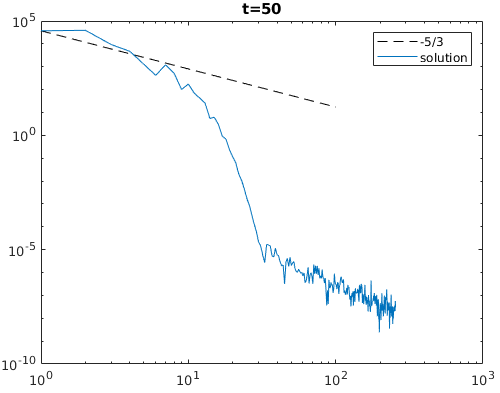
\includegraphics[width=4.5cm]{Figs/ns_t50_n3_spectra.png}
    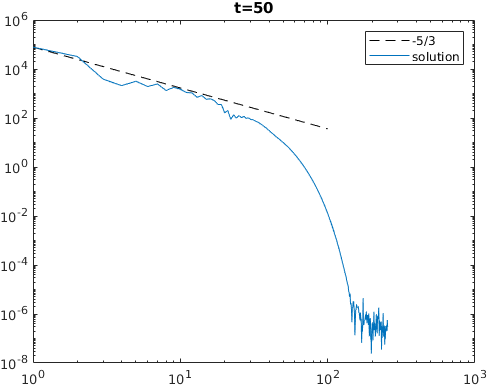
\includegraphics[width=4.5cm]{Figs/ns_t50_n4_spectra.png}
    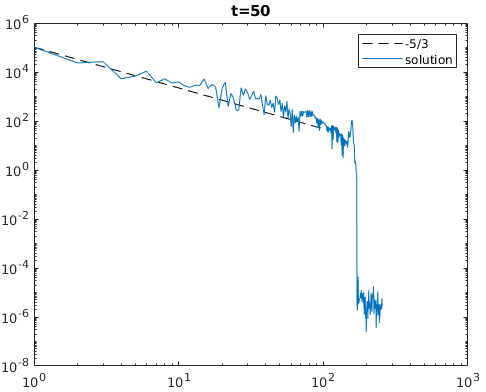
\includegraphics[width=4.5cm]{Figs/ns_t50_n5_spectra.png}
    \caption{Spectral Decay of Navier-Stokes.}
    \label{fig:spectral1}
    \small{ The spectral decay of the Navier-stokes equation data. The y-axis is represents the value of each mode; the x-axis is the wavenumber $|k| = k_1 + k_2$. From left to right, the solutions have viscosity \(\nu = 10^{-3}, \: 10^{-4}, \: 10^{-5}\) respectively.}
\end{figure}

\subsection{Choice of Loss Criteria}
In general, the model has the best performance when trained and tested using the same loss criteria. If one trains the model using one norm and tests with another norm, the model may overfit in the training norm. Furthermore, the choice of loss function plays a key role.
In this work, we use the relative $L_2$ error to measure the performance in all our problems. Both the $L_2$ error and its square, the mean squared error (MSE), are common choices of the testing criteria in the numerical analysis and machine learning literature. We observed that using the relative error to train the model has a good normalization and regularization effect that prevents overfitting. In practice, training with the relative $L_2$ loss results in around half the testing error rate compared to training with the MSE loss.